\section{Topic}
\label{s:topic} % This declares a label so you can reference the section elsewhere.

Talk about your main points here.
Perhaps add additional sections as necessary to break it into logical sections.
Good stuff.

\subsection{Information}

This is a bulleted list:
\begin{itemize}
\item Item 1
\item Item 2
\item Item 3
\item Item 4
\end{itemize}

This is a numbered list:
\begin{enumerate}
\item Item 1
\item Item 2
\item Item 3
\item Item 4
\end{enumerate}

\subsection{How to make a figure}
Sometimes you want figures in your paper.
Use the includegraphics command to insert figures, like in Figure~\ref{f:os_block}.

\begin{figure}
\centering % Make it center
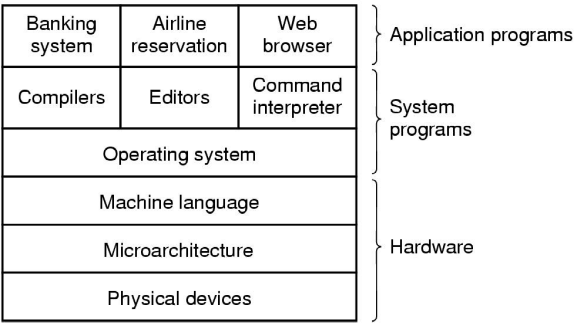
\includegraphics[width=0.5\textwidth]{figures/os_block.png}
\caption{This is a caption for the figure}
\label{f:os_block}
\end{figure}

\subsection{How to include a table}
Tables are created using the tabular environment.
You can see it in Table~\ref{t:my_table}.

\begin{table}
\centering % Make it center
\begin{tabular}{l|cc} % Second argument is column list, one character per.  Justify with lcr.  Pipe for horizontal line
Name & Col 1 & Col 2 \\ % Separate columns with &, end line with \\
\hline % Horizontal line
Item 1 & 1 & 2 \\
Item 2 & 3 & 4\\
\end{tabular}
\caption{This is a caption for the table}
\label{t:my_table}
\end{table}

\subsection{More Fake Text}
More fake text here, but in subsections.

\subsubsection{Fizz}
\lipsum[6-8]

\subsubsection{Buzz}
\lipsum[9-10]
